%%%%%%%%%%%%%%%%%%%%%%%%%%%%%%%%%%%%%%%%%%%%%%%%%%%%%%%%%%%%%%%%%%%%%%%%%%%%%%%%%%
\begin{frame}[fragile]\frametitle{Tadasana}
\begin{columns}
    \begin{column}[T]{0.5\linewidth}
      \begin{itemize}
        \item Stand with feet together, arms by sides.
        \item Distribute weight evenly on both feet.
        \item Engage thighs and lift chest.
        \item Extend arms overhead, palms facing each other.
        \item Hold the pose and breathe deeply.
        \item \textbf{Benefits:} Improves posture, strengthens legs, and enhances concentration.
        \item \textbf{Contraindications:} Avoid if you have low blood pressure or are recovering from surgery.
      \end{itemize}
    \end{column}
    \begin{column}[T]{0.5\linewidth}
        \begin{center}
		        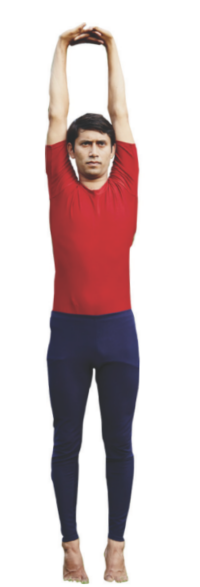
\includegraphics[width=0.35\linewidth,keepaspectratio]{ycb1_tadasan}
				
				{\tiny (Ref: Certification  of Yoga Professionals Official Guidebook For Level I (Instructor))}		
        \end{center}    
    \end{column}
  \end{columns}
\end{frame}

%%%%%%%%%%%%%%%%%%%%%%%%%%%%%%%%%%%%%%%%%%%%%%%%%%%%%%%%%%%%%%%%%%%%%%%%%%%%%%%%%%
\begin{frame}[fragile]\frametitle{Vrikshasana}
\begin{columns}
    \begin{column}[T]{0.5\linewidth}
      \begin{itemize}
        \item Stand in Tadasana position.
        \item Shift weight to one foot, bend the other knee.
        \item Place the sole of the bent foot on the inner thigh of the standing leg.
        \item Join hands in front of the chest or extend overhead.
        \item Hold the position, focus on balance.
        \item \textbf{Benefits:} Enhances balance, strengthens legs, and improves concentration.
        \item \textbf{Contraindications:} Avoid if you have knee or ankle injuries.
      \end{itemize}
    \end{column}
    \begin{column}[T]{0.5\linewidth}
        \begin{center}
		        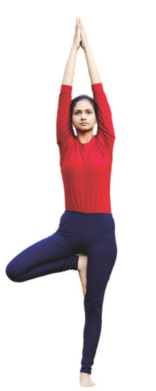
\includegraphics[width=0.4\linewidth,keepaspectratio]{ycb1_vrikshasan}
				
				{\tiny (Ref: Certification  of Yoga Professionals Official Guidebook For Level I (Instructor))}	        
		\end{center}    
    \end{column}
  \end{columns}
\end{frame}

%%%%%%%%%%%%%%%%%%%%%%%%%%%%%%%%%%%%%%%%%%%%%%%%%%%%%%%%%%%%%%%%%%%%%%%%%%%%%%%%%%
\begin{frame}[fragile]\frametitle{Ardha Chakrasana or Hastottanasan}
\begin{columns}
    \begin{column}[T]{0.5\linewidth}
      \begin{itemize}
        \item Stand with feet shoulder-width apart.
        \item Place hands on lower back for support.
        \item Inhale and lift chest, pressing hips forward.
        \item Exhale and gently arch the back.
        \item Hold the pose, breathing deeply.
        \item \textbf{Benefits:} Stretches spine, improves posture, and relieves back pain.
        \item \textbf{Contraindications:} Avoid if you have back injuries or abdominal issues.
      \end{itemize}
    \end{column}
    \begin{column}[T]{0.5\linewidth}
        \begin{center}
        \begin{center}
		        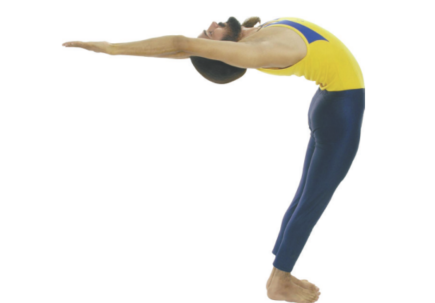
\includegraphics[width=\linewidth,keepaspectratio]{ycb1_ardhachakrasan}
				
				{\tiny (Ref: Certification  of Yoga Professionals Official Guidebook For Level I (Instructor))}	        
		\end{center}   
        \end{center}    
    \end{column}
  \end{columns}
\end{frame}

%%%%%%%%%%%%%%%%%%%%%%%%%%%%%%%%%%%%%%%%%%%%%%%%%%%%%%%%%%%%%%%%%%%%%%%%%%%%%%%%%%
\begin{frame}[fragile]\frametitle{Padahastasana}
\begin{columns}
    \begin{column}[T]{0.5\linewidth}
      \begin{itemize}
        \item Stand with feet together, arms by sides.
        \item Inhale and raise arms overhead.
        \item Exhale and bend forward, reaching for the feet.
        \item Keep knees slightly bent if needed.
        \item Hold the pose and breathe deeply.
        \item \textbf{Benefits:} Stretches hamstrings, improves flexibility, and calms the mind.
        \item \textbf{Contraindications:} Avoid if you have back or hamstring injuries.
      \end{itemize}
    \end{column}
    \begin{column}[T]{0.5\linewidth}
        \begin{center}
        \begin{center}
		        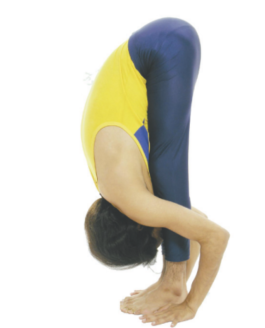
\includegraphics[width=0.9\linewidth,keepaspectratio]{ycb1_padahastasan}
				
				{\tiny (Ref: Certification  of Yoga Professionals Official Guidebook For Level I (Instructor))}	        
		\end{center}   
        \end{center}    
    \end{column}
  \end{columns}
\end{frame}

%%%%%%%%%%%%%%%%%%%%%%%%%%%%%%%%%%%%%%%%%%%%%%%%%%%%%%%%%%%%%%%%%%%%%%%%%%%%%%%%%%
\begin{frame}[fragile]\frametitle{Kati Chakrasana}
\begin{columns}
    \begin{column}[T]{0.5\linewidth}
      \begin{itemize}
        \item Stand with feet shoulder-width apart, arms outstretched.
        \item Twist torso to one side, bringing opposite hand to shoulder.
        \item Hold the twist, then return to center.
        \item Repeat on the other side.
        \item Breathe deeply during each twist.
        \item \textbf{Benefits:} Enhances spinal flexibility, massages abdominal organs, and improves digestion.
        \item \textbf{Contraindications:} Avoid if you have back or spinal issues.
      \end{itemize}
    \end{column}
    \begin{column}[T]{0.5\linewidth}
        \begin{center}
        \begin{center}
		        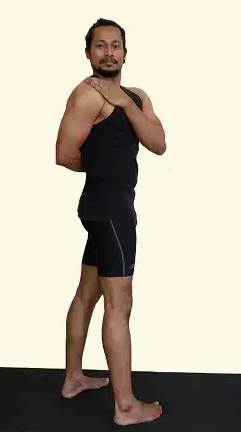
\includegraphics[width=0.6\linewidth,keepaspectratio]{ycb1_katichakrasan}
				
				{\tiny (Ref: Prana Yoga)}	        
		\end{center}   
        \end{center}    
    \end{column}
  \end{columns}
\end{frame}

%%%%%%%%%%%%%%%%%%%%%%%%%%%%%%%%%%%%%%%%%%%%%%%%%%%%%%%%%%%%%%%%%%%%%%%%%%%%%%%%%%
\begin{frame}[fragile]\frametitle{Trikonasana}
\begin{columns}
    \begin{column}[T]{0.5\linewidth}
      \begin{itemize}
        \item Stand with feet wide apart, arms extended.
        \item Turn one foot out and the other foot slightly in.
        \item Reach towards the foot, placing hand on ankle or shin.
        \item Extend the other arm upwards, gaze up.
        \item Hold the position, then switch sides.
        \item \textbf{Benefits:} Stretches legs, improves balance, and strengthens core.
        \item \textbf{Contraindications:} Avoid if you have leg or back injuries.
      \end{itemize}
    \end{column}
    \begin{column}[T]{0.5\linewidth}
        \begin{center}
        \begin{center}
		        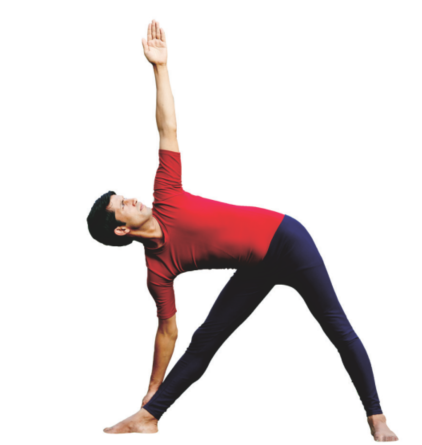
\includegraphics[width=\linewidth,keepaspectratio]{ycb1_trikonasan}
				
				{\tiny (Ref: Certification  of Yoga Professionals Official Guidebook For Level I (Instructor))}	        
		\end{center}   
        \end{center}    
    \end{column}
  \end{columns}
\end{frame}

%%%%%%%%%%%%%%%%%%%%%%%%%%%%%%%%%%%%%%%%%%%%%%%%%%%%%%%%%%%%%%%%%%%%%%%%%%%%%%%%%%
\begin{frame}[fragile]\frametitle{Dandasana}
\begin{columns}
    \begin{column}[T]{0.5\linewidth}
      \begin{itemize}
        \item Sit with legs extended, feet flexed.
        \item Keep spine straight and shoulders relaxed.
        \item Place hands beside hips, fingers pointing forward.
        \item Engage thigh muscles and lift chest.
        \item Hold the pose, breathing steadily.
        \item \textbf{Benefits:} Strengthens back and legs, improves posture, and calms the mind.
        \item \textbf{Contraindications:} Avoid if you have lower back pain or hamstring injuries.
      \end{itemize}
    \end{column}
    \begin{column}[T]{0.5\linewidth}
        \begin{center}
        \begin{center}
		        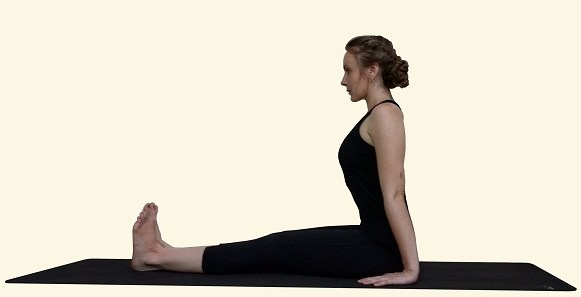
\includegraphics[width=\linewidth,keepaspectratio]{ycb1_dandasan}
				
				{\tiny (Ref: Prana Yoga)}	        
		\end{center}   
        \end{center}    
    \end{column}
  \end{columns}
\end{frame}

%%%%%%%%%%%%%%%%%%%%%%%%%%%%%%%%%%%%%%%%%%%%%%%%%%%%%%%%%%%%%%%%%%%%%%%%%%%%%%%%%%
\begin{frame}[fragile]\frametitle{Sukhasana}
\begin{columns}
    \begin{column}[T]{0.5\linewidth}
      \begin{itemize}
        \item Sit with legs crossed comfortably.
        \item Place hands on knees or in a mudra.
        \item Keep spine upright and shoulders relaxed.
        \item Close eyes and focus on breath.
        \item Hold the position, breathing deeply.
        \item \textbf{Benefits:} Promotes relaxation, improves flexibility, and calms the mind.
        \item \textbf{Contraindications:} Avoid if you have knee or hip injuries.
      \end{itemize}
    \end{column}
    \begin{column}[T]{0.5\linewidth}
        \begin{center}
        \begin{center}
		        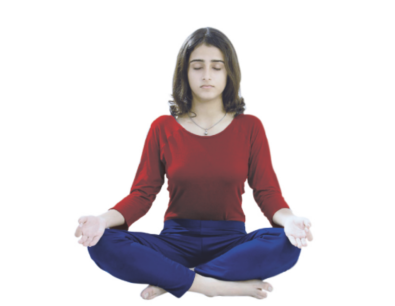
\includegraphics[width=\linewidth,keepaspectratio]{ycb1_sukhasan}
				
				{\tiny (Ref: Certification  of Yoga Professionals Official Guidebook For Level I (Instructor))}	        
		\end{center}   
        \end{center}    
    \end{column}
  \end{columns}
\end{frame}

%%%%%%%%%%%%%%%%%%%%%%%%%%%%%%%%%%%%%%%%%%%%%%%%%%%%%%%%%%%%%%%%%%%%%%%%%%%%%%%%%%
\begin{frame}[fragile]\frametitle{Padmasana}
\begin{columns}
    \begin{column}[T]{0.5\linewidth}
      \begin{itemize}
        \item Sit with legs extended, then bend one knee.
        \item Place the foot on the opposite thigh.
        \item Repeat with the other leg, placing the foot on the opposite thigh.
        \item Keep spine straight and shoulders relaxed.
        \item Hold the position, focusing on breath.
        \item \textbf{Benefits:} Enhances meditation, stretches hips, and calms the mind.
        \item \textbf{Contraindications:} Avoid if you have knee or hip injuries.
      \end{itemize}
    \end{column}
    \begin{column}[T]{0.5\linewidth}
        \begin{center}
        \begin{center}
		        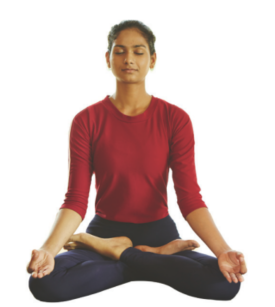
\includegraphics[width=\linewidth,keepaspectratio]{ycb1_padmasan}
				
				{\tiny (Ref: Certification  of Yoga Professionals Official Guidebook For Level I (Instructor))}	        
		\end{center}   
        \end{center}    
    \end{column}
  \end{columns}
\end{frame}

%%%%%%%%%%%%%%%%%%%%%%%%%%%%%%%%%%%%%%%%%%%%%%%%%%%%%%%%%%%%%%%%%%%%%%%%%%%%%%%%%%
\begin{frame}[fragile]\frametitle{Vajrasana}
\begin{columns}
    \begin{column}[T]{0.5\linewidth}
      \begin{itemize}
        \item Kneel on the floor, sit back on heels.
        \item Keep thighs perpendicular to the floor.
        \item Place hands on knees, palms facing down.
        \item Keep spine straight and shoulders relaxed.
        \item Breathe deeply, holding the position.
        \item \textbf{Benefits:} Aids digestion, relieves lower back pain, and improves posture.
        \item \textbf{Contraindications:} Avoid if you have knee or ankle injuries.
      \end{itemize}
    \end{column}
    \begin{column}[T]{0.5\linewidth}
        \begin{center}
        \begin{center}
		        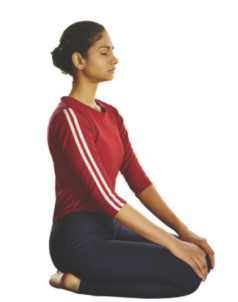
\includegraphics[width=0.8\linewidth,keepaspectratio]{ycb1_vajrasan}
				
				{\tiny (Ref: Certification  of Yoga Professionals Official Guidebook For Level I (Instructor))}	        
		\end{center}   
        \end{center}    
    \end{column}
  \end{columns}
\end{frame}

%%%%%%%%%%%%%%%%%%%%%%%%%%%%%%%%%%%%%%%%%%%%%%%%%%%%%%%%%%%%%%%%%%%%%%%%%%%%%%%%%%
\begin{frame}[fragile]\frametitle{Bhadrasana}
\begin{columns}
    \begin{column}[T]{0.5\linewidth}
      \begin{itemize}
        \item Sit with legs extended, then bend knees and bring feet together.
        \item Place feet close to the pelvis, holding toes with hands.
        \item Press knees gently towards the floor.
        \item Keep spine erect and shoulders relaxed.
        \item Hold the pose and breathe deeply.
        \item \textbf{Benefits:} Opens hips, improves flexibility, and calms the mind.
        \item \textbf{Contraindications:} Avoid if you have knee or hip injuries.
      \end{itemize}
    \end{column}
    \begin{column}[T]{0.5\linewidth}
        \begin{center}
        \begin{center}
		        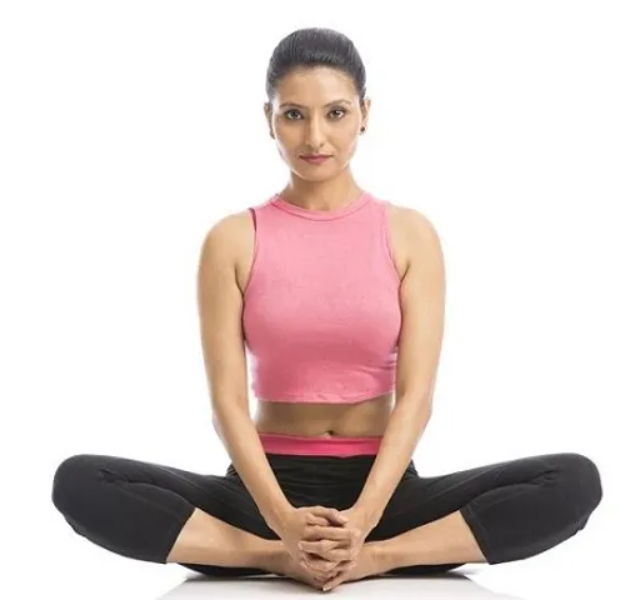
\includegraphics[width=\linewidth,keepaspectratio]{ycb1_bhadrasan}
				
				{\tiny (Ref: Patanjali Japan Foundation)}	        
		\end{center}   
        \end{center}    
    \end{column}
  \end{columns}
\end{frame}

%%%%%%%%%%%%%%%%%%%%%%%%%%%%%%%%%%%%%%%%%%%%%%%%%%%%%%%%%%%%%%%%%%%%%%%%%%%%%%%%%%
\begin{frame}[fragile]\frametitle{Mandukasana}
\begin{columns}
    \begin{column}[T]{0.5\linewidth}
      \begin{itemize}
        \item Start in a kneeling position, sit on heels.
        \item Place palms together in front of the chest.
        \item Inhale and stretch arms forward, keeping palms together.
        \item Exhale and bring hands back to the chest.
        \item Repeat the sequence.
        \item \textbf{Benefits:} Improves flexibility of hips and thighs, enhances focus.
        \item \textbf{Contraindications:} Avoid if you have knee or back issues.
      \end{itemize}
    \end{column}
    \begin{column}[T]{0.5\linewidth}
        \begin{center}
        \begin{center}
		        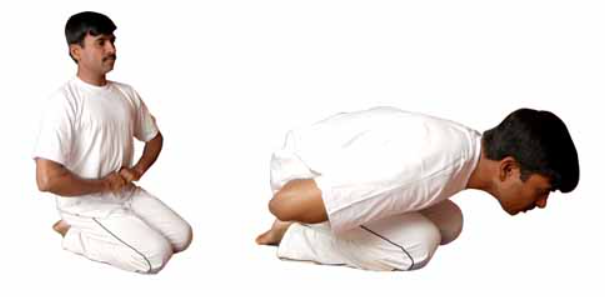
\includegraphics[width=\linewidth,keepaspectratio]{ycb1_mandukasan}
				
				{\tiny (Ref: Atma Bodh)}	        
		\end{center}   
        \end{center}    
    \end{column}
  \end{columns}
\end{frame}

%%%%%%%%%%%%%%%%%%%%%%%%%%%%%%%%%%%%%%%%%%%%%%%%%%%%%%%%%%%%%%%%%%%%%%%%%%%%%%%%%%
\begin{frame}[fragile]\frametitle{Ushtrasana}
\begin{columns}
    \begin{column}[T]{0.5\linewidth}
      \begin{itemize}
        \item Kneel with knees hip-width apart.
        \item Place hands on lower back for support.
        \item Inhale and lift chest, arching back.
        \item Reach for heels with hands, if possible.
        \item Hold the position, breathing deeply.
        \item \textbf{Benefits:} Stretches the entire front body, opens chest, and improves posture.
        \item \textbf{Contraindications:} Avoid if you have back or neck issues.
      \end{itemize}
    \end{column}
    \begin{column}[T]{0.5\linewidth}
        \begin{center}
        \begin{center}
		        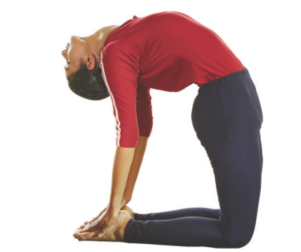
\includegraphics[width=\linewidth,keepaspectratio]{ycb1_ushtrasan}
				
				{\tiny (Ref: Certification  of Yoga Professionals Official Guidebook For Level I (Instructor))}	        
		\end{center}   
        \end{center}    
    \end{column}
  \end{columns}
\end{frame}

%%%%%%%%%%%%%%%%%%%%%%%%%%%%%%%%%%%%%%%%%%%%%%%%%%%%%%%%%%%%%%%%%%%%%%%%%%%%%%%%%%
\begin{frame}[fragile]\frametitle{Shashankasana}
\begin{columns}
    \begin{column}[T]{0.5\linewidth}
      \begin{itemize}
        \item Kneel and sit on heels.
        \item Extend arms forward on the floor.
        \item Rest forehead on the ground.
        \item Hold the position, breathing deeply.
        \item \textbf{Benefits:} Relieves stress, stretches back and thighs.
        \item \textbf{Contraindications:} Avoid if you have knee or back injuries.
      \end{itemize}
    \end{column}
    \begin{column}[T]{0.5\linewidth}
        \begin{center}
        \begin{center}
		        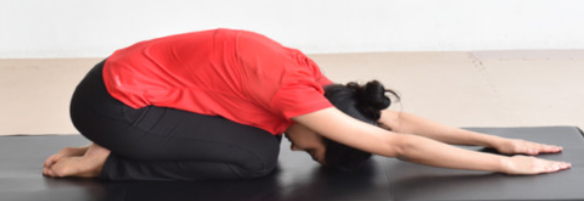
\includegraphics[width=\linewidth,keepaspectratio]{ycb1_shashankasan}
				
				{\tiny (Ref: Certification  of Yoga Professionals Official Guidebook For Level I (Instructor))}	        
		\end{center}   
        \end{center}    
    \end{column}
  \end{columns}
\end{frame}

%%%%%%%%%%%%%%%%%%%%%%%%%%%%%%%%%%%%%%%%%%%%%%%%%%%%%%%%%%%%%%%%%%%%%%%%%%%%%%%%%%
\begin{frame}[fragile]\frametitle{Uttana Mandukasana}
\begin{columns}
    \begin{column}[T]{0.5\linewidth}
      \begin{itemize}
        \item Start in Mandukasana position.
        \item Bend forward from hips, extending arms forward.
        \item Rest forehead on the floor, keep arms extended.
        \item Hold the position, breathing deeply.
        \item \textbf{Benefits:} Enhances spinal flexibility, stretches back and thighs.
        \item \textbf{Contraindications:} Avoid if you have knee or back injuries.
      \end{itemize}
    \end{column}
    \begin{column}[T]{0.5\linewidth}
        \begin{center}
        \begin{center}
		        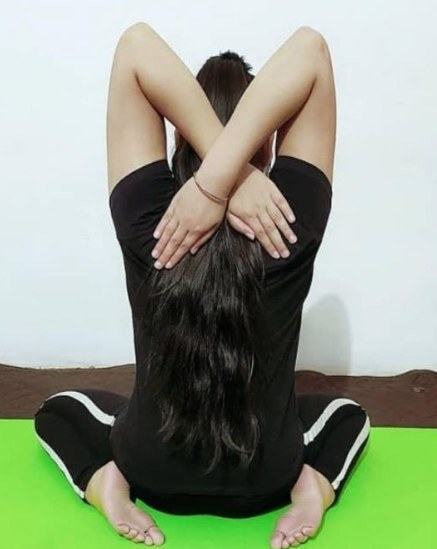
\includegraphics[width=0.9\linewidth,keepaspectratio]{ycb1_uttanamandukasan}
				
				{\tiny (Ref: Certification  of Yoga Professionals Official Guidebook For Level I (Instructor))}	        
		\end{center}   
        \end{center}    
    \end{column}
  \end{columns}
\end{frame}

%%%%%%%%%%%%%%%%%%%%%%%%%%%%%%%%%%%%%%%%%%%%%%%%%%%%%%%%%%%%%%%%%%%%%%%%%%%%%%%%%%
\begin{frame}[fragile]\frametitle{Paschimottanasana}
\begin{columns}
    \begin{column}[T]{0.5\linewidth}
      \begin{itemize}
        \item Sit with legs extended, feet flexed.
        \item Inhale and lengthen spine.
        \item Exhale and bend forward, reaching for feet.
        \item Hold the pose and breathe deeply.
        \item \textbf{Benefits:} Stretches the spine and hamstrings, calms the mind.
        \item \textbf{Contraindications:} Avoid if you have back or hamstring injuries.
      \end{itemize}
    \end{column}
    \begin{column}[T]{0.5\linewidth}
        \begin{center}
        \begin{center}
		        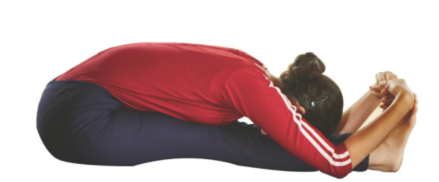
\includegraphics[width=\linewidth,keepaspectratio]{ycb1_pashchimottansasan}
				
				{\tiny (Ref: Certification  of Yoga Professionals Official Guidebook For Level I (Instructor))}	        
		\end{center}   
        \end{center}    
    \end{column}
  \end{columns}
\end{frame}

%%%%%%%%%%%%%%%%%%%%%%%%%%%%%%%%%%%%%%%%%%%%%%%%%%%%%%%%%%%%%%%%%%%%%%%%%%%%%%%%%%
\begin{frame}[fragile]\frametitle{Purvottanasana}
\begin{columns}
    \begin{column}[T]{0.5\linewidth}
      \begin{itemize}
        \item Sit with legs extended and hands behind hips.
        \item Inhale and lift hips off the floor, pressing palms into the ground.
        \item Open chest and face upward.
        \item Hold the pose and breathe deeply.
        \item \textbf{Benefits:} Strengthens arms and shoulders, stretches chest and front body.
        \item \textbf{Contraindications:} Avoid if you have wrist or shoulder injuries.
      \end{itemize}
    \end{column}
    \begin{column}[T]{0.5\linewidth}
        \begin{center}
        \begin{center}
		        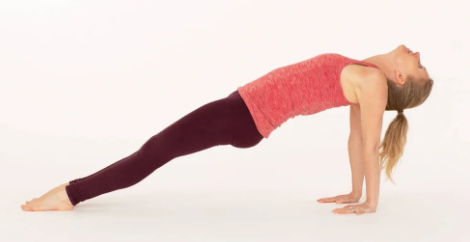
\includegraphics[width=\linewidth,keepaspectratio]{ycb1_purvottansasan}
				
				{\tiny (Ref: Ekhart Yoga)}	        
		\end{center}   
        \end{center}    
    \end{column}
  \end{columns}
\end{frame}

%%%%%%%%%%%%%%%%%%%%%%%%%%%%%%%%%%%%%%%%%%%%%%%%%%%%%%%%%%%%%%%%%%%%%%%%%%%%%%%%%%
\begin{frame}[fragile]\frametitle{Vakrasana}
\begin{columns}
    \begin{column}[T]{0.5\linewidth}
      \begin{itemize}
        \item Sit with legs extended and back straight.
        \item Bend one knee and place the foot on the outside of the opposite thigh.
        \item Twist torso towards the bent knee, placing the opposite elbow on the knee.
        \item Hold the twist, then switch sides.
        \item \textbf{Benefits:} Enhances spinal flexibility, massages abdominal organs.
        \item \textbf{Contraindications:} Avoid if you have spinal or abdominal issues.
      \end{itemize}
    \end{column}
    \begin{column}[T]{0.5\linewidth}
        \begin{center}
        \begin{center}
		        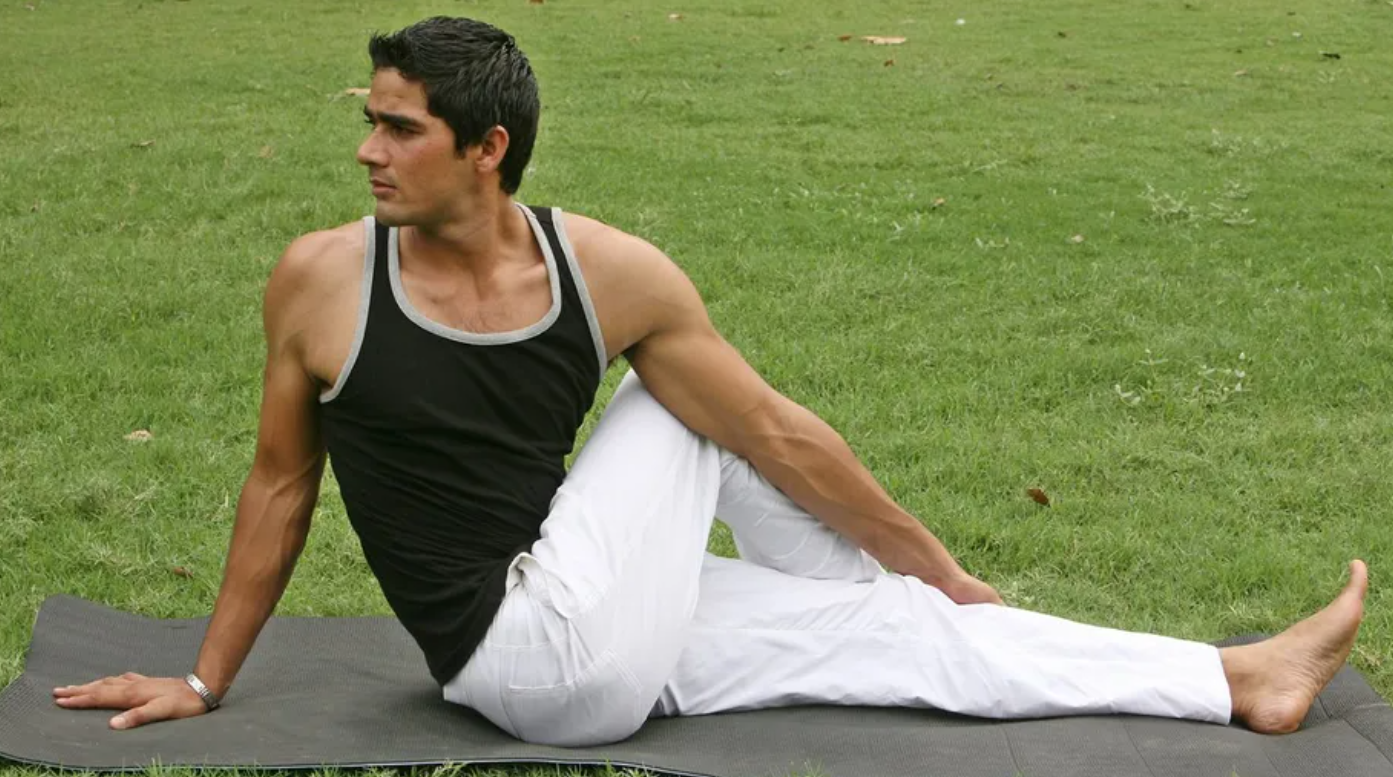
\includegraphics[width=\linewidth,keepaspectratio]{ycb1_vakrasan}
				
				{\tiny (Ref: CONDE NAST TRAVELLER)}	        
		\end{center}   
        \end{center}    
    \end{column}
  \end{columns}
\end{frame}

%%%%%%%%%%%%%%%%%%%%%%%%%%%%%%%%%%%%%%%%%%%%%%%%%%%%%%%%%%%%%%%%%%%%%%%%%%%%%%%%%%
\begin{frame}[fragile]\frametitle{Gomukhasana}
\begin{columns}
    \begin{column}[T]{0.5\linewidth}
      \begin{itemize}
        \item Sit with legs crossed, one knee stacked on top of the other.
        \item Bring one arm behind the back, and the other arm over the shoulder.
        \item Join hands behind the back if possible.
        \item Hold the pose and breathe deeply.
        \item \textbf{Benefits:} Stretches shoulders, hips, and thighs.
        \item \textbf{Contraindications:} Avoid if you have shoulder or knee injuries.
      \end{itemize}
    \end{column}
    \begin{column}[T]{0.5\linewidth}
        \begin{center}
        \begin{center}
		        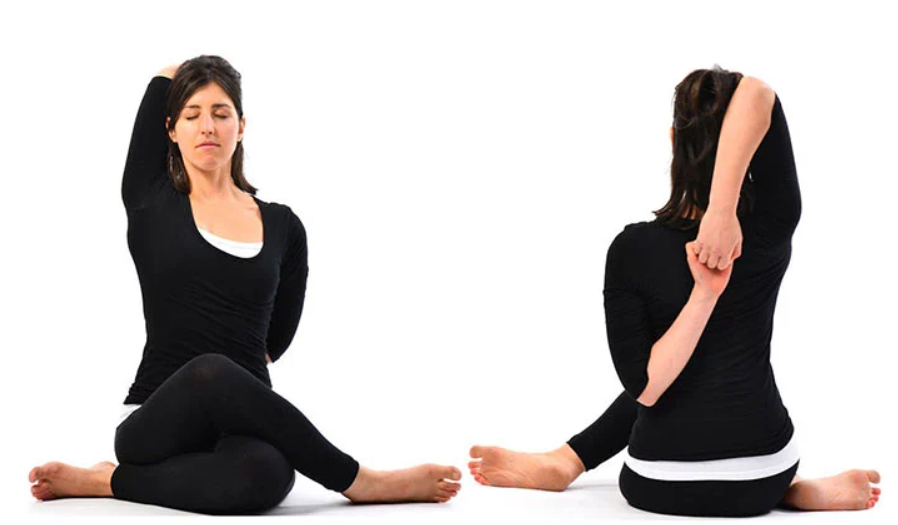
\includegraphics[width=\linewidth,keepaspectratio]{ycb1_gomukhasan}
				
				{\tiny (Ref: Himalayan Yoga Ashram)}	        
		\end{center}   
        \end{center}    
    \end{column}
  \end{columns}
\end{frame}

%%%%%%%%%%%%%%%%%%%%%%%%%%%%%%%%%%%%%%%%%%%%%%%%%%%%%%%%%%%%%%%%%%%%%%%%%%%%%%%%%%
\begin{frame}[fragile]\frametitle{Bhujangasana}
\begin{columns}
    \begin{column}[T]{0.5\linewidth}
      \begin{itemize}
        \item Lie on your stomach, legs extended, and feet together.
        \item Place hands under shoulders, elbows close to the body.
        \item Inhale and lift chest, keeping the navel on the floor.
        \item Hold the pose and breathe deeply.
        \item \textbf{Benefits:} Strengthens back, stretches chest and shoulders.
        \item \textbf{Contraindications:} Avoid if you have back or wrist injuries.
      \end{itemize}
    \end{column}
    \begin{column}[T]{0.5\linewidth}
        \begin{center}
        \begin{center}
		        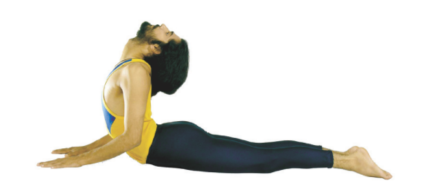
\includegraphics[width=\linewidth,keepaspectratio]{ycb1_bhujangasan}
				
				{\tiny (Ref: Certification  of Yoga Professionals Official Guidebook For Level I (Instructor))}	        
		\end{center}   
        \end{center}    
    \end{column}
  \end{columns}
\end{frame}

%%%%%%%%%%%%%%%%%%%%%%%%%%%%%%%%%%%%%%%%%%%%%%%%%%%%%%%%%%%%%%%%%%%%%%%%%%%%%%%%%%
\begin{frame}[fragile]\frametitle{Shalabhasana}
\begin{columns}
    \begin{column}[T]{0.5\linewidth}
      \begin{itemize}
        \item Lie on your stomach, arms by sides.
        \item Inhale and lift legs and chest off the floor.
        \item Keep arms and feet active.
        \item Hold the position, breathing deeply.
        \item \textbf{Benefits:} Strengthens lower back, improves posture.
        \item \textbf{Contraindications:} Avoid if you have back or abdominal issues.
      \end{itemize}
    \end{column}
    \begin{column}[T]{0.5\linewidth}
        \begin{center}
        \begin{center}
		        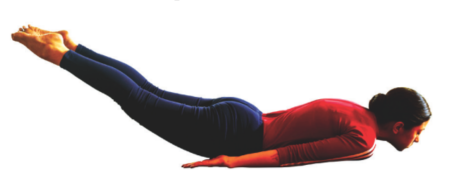
\includegraphics[width=\linewidth,keepaspectratio]{ycb1_shalabhasan}
				
				{\tiny (Ref: Certification  of Yoga Professionals Official Guidebook For Level I (Instructor))}	        
		\end{center}   
        \end{center}    
    \end{column}
  \end{columns}
\end{frame}

%%%%%%%%%%%%%%%%%%%%%%%%%%%%%%%%%%%%%%%%%%%%%%%%%%%%%%%%%%%%%%%%%%%%%%%%%%%%%%%%%%
\begin{frame}[fragile]\frametitle{Makarasana}
\begin{columns}
    \begin{column}[T]{0.5\linewidth}
      \begin{itemize}
        \item Lie on your stomach, arms extended to sides.
        \item Bend knees and place feet on the floor.
        \item Rest forehead on the hands or ground.
        \item Breathe deeply and relax.
        \item \textbf{Benefits:} Relieves back pain, relaxes spine.
        \item \textbf{Contraindications:} None.
      \end{itemize}
    \end{column}
    \begin{column}[T]{0.5\linewidth}
        \begin{center}
        \begin{center}
		        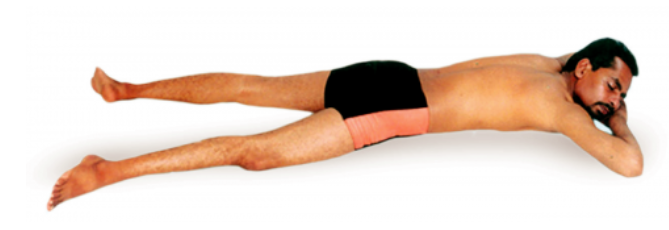
\includegraphics[width=\linewidth,keepaspectratio]{ycb1_makarasan}
				
				{\tiny (Ref: Vydya Health)}	        
		\end{center}   
        \end{center}    
    \end{column}
  \end{columns}
\end{frame}

%%%%%%%%%%%%%%%%%%%%%%%%%%%%%%%%%%%%%%%%%%%%%%%%%%%%%%%%%%%%%%%%%%%%%%%%%%%%%%%%%%
\begin{frame}[fragile]\frametitle{Pavanamuktasana}
\begin{columns}
    \begin{column}[T]{0.5\linewidth}
      \begin{itemize}
        \item Lie on your back, knees bent, and feet on the floor.
        \item Hug knees to chest, interlace fingers around shins.
        \item Lift head and shoulders off the floor.
        \item Hold the position and breathe deeply.
        \item \textbf{Benefits:} Relieves gas, massages abdominal organs.
        \item \textbf{Contraindications:} Avoid if you have back issues or are pregnant.
      \end{itemize}
    \end{column}
    \begin{column}[T]{0.5\linewidth}
        \begin{center}
        \begin{center}
		        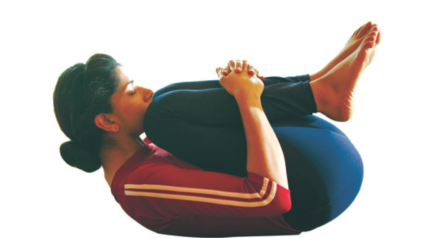
\includegraphics[width=\linewidth,keepaspectratio]{ycb1_pavanamuktasan}
				
				{\tiny (Ref: Certification  of Yoga Professionals Official Guidebook For Level I (Instructor))}	        
		\end{center}   
        \end{center}    
    \end{column}
  \end{columns}
\end{frame}

%%%%%%%%%%%%%%%%%%%%%%%%%%%%%%%%%%%%%%%%%%%%%%%%%%%%%%%%%%%%%%%%%%%%%%%%%%%%%%%%%%
\begin{frame}[fragile]\frametitle{Uttanapadasana / Ardha Halasana}
\begin{columns}
    \begin{column}[T]{0.5\linewidth}
      \begin{itemize}
        \item Lie on your back, legs extended, and arms by sides.
        \item Inhale and lift legs to a 45-degree angle.
        \item Keep back and shoulders on the floor.
        \item Hold the position and breathe deeply.
        \item \textbf{Benefits:} Strengthens abdominal muscles, tones legs.
        \item \textbf{Contraindications:} Avoid if you have back or leg issues.
      \end{itemize}
    \end{column}
    \begin{column}[T]{0.5\linewidth}
        \begin{center}
        \begin{center}
		        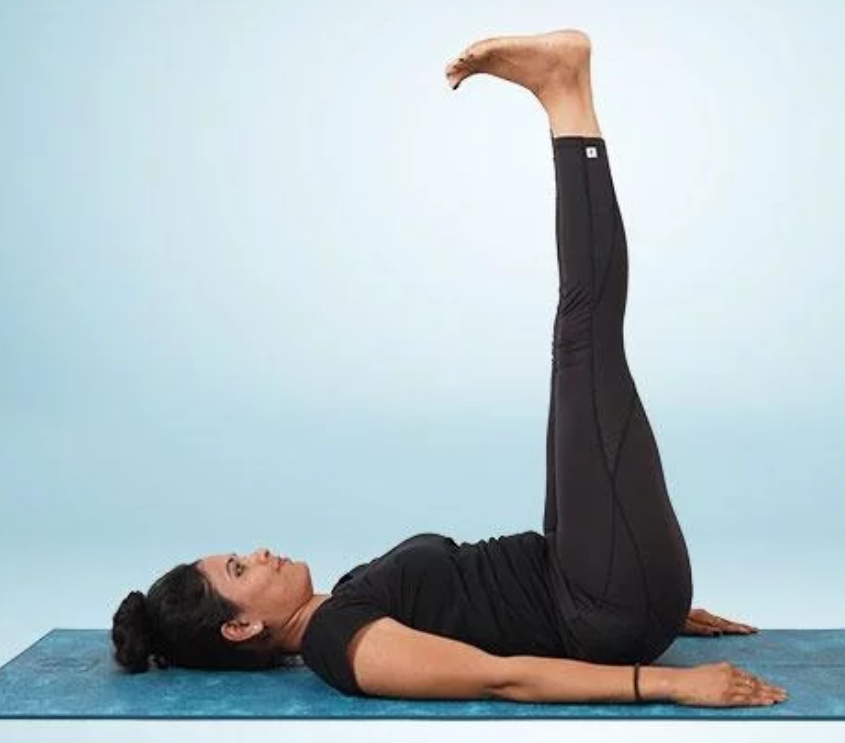
\includegraphics[width=\linewidth,keepaspectratio]{ycb1_uttanpadasan}
				
				{\tiny (Ref: Bodhi School of Yoga)}	        
		\end{center}   
        \end{center}    
    \end{column}
  \end{columns}
\end{frame}

% %%%%%%%%%%%%%%%%%%%%%%%%%%%%%%%%%%%%%%%%%%%%%%%%%%%%%%%%%%%%%%%%%%%%%%%%%%%%%%%%%%
% \begin{frame}[fragile]\frametitle{}
% \begin{columns}
    % \begin{column}[T]{0.5\linewidth}
      % \begin{itemize}
        % \item Lie on your back, arms by sides.
        % \item Lift legs overhead, bringing toes to the floor behind the head.
        % \item Support lower back with hands if needed.
        % \item Hold the position and breathe deeply.
        % \item \textbf{Benefits:} Stretches back and legs, strengthens core.
        % \item \textbf{Contraindications:} Avoid if you have neck or back issues.
      % \end{itemize}
    % \end{column}
    % \begin{column}[T]{0.5\linewidth}
        % \begin{center}
        % \begin{center}
		        % 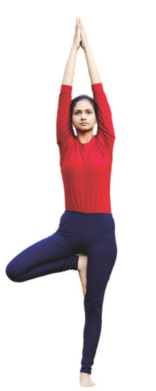
\includegraphics[width=\linewidth,keepaspectratio]{ycb1_vrikshasan}
				
				% {\tiny (Ref: Certification  of Yoga Professionals Official Guidebook For Level I (Instructor))}	        
		% \end{center}   
        % \end{center}    
    % \end{column}
  % \end{columns}
% \end{frame}

%%%%%%%%%%%%%%%%%%%%%%%%%%%%%%%%%%%%%%%%%%%%%%%%%%%%%%%%%%%%%%%%%%%%%%%%%%%%%%%%%%
\begin{frame}[fragile]\frametitle{Setubandhasana}
\begin{columns}
    \begin{column}[T]{0.5\linewidth}
      \begin{itemize}
        \item Lie on your back, knees bent, feet on the floor.
        \item Lift hips towards the ceiling, pressing into feet.
        \item Interlace fingers under back for support.
        \item Hold the position and breathe deeply.
        \item \textbf{Benefits:} Strengthens back and legs, stretches chest.
        \item \textbf{Contraindications:} Avoid if you have neck or back injuries.
      \end{itemize}
    \end{column}
    \begin{column}[T]{0.5\linewidth}
        \begin{center}
        \begin{center}
		        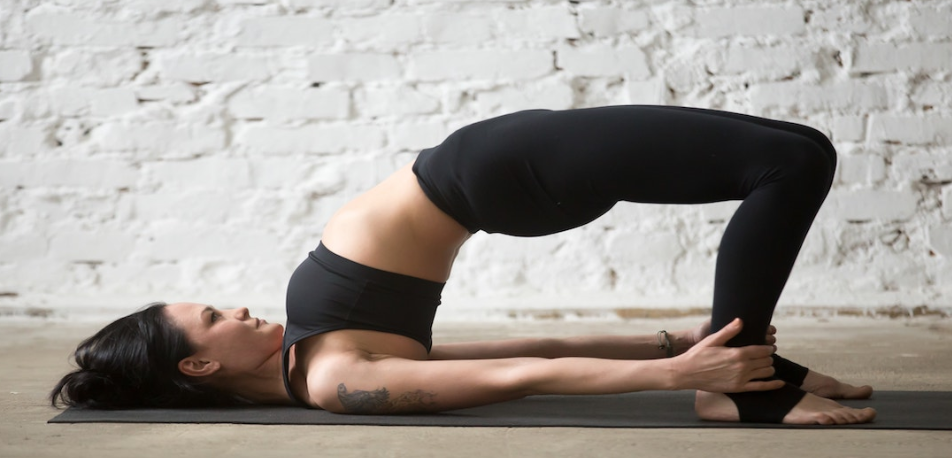
\includegraphics[width=\linewidth,keepaspectratio]{ycb1_setubandhasan}
				
				{\tiny (Ref: Rishikesh Yogis Yogashala)}	        
		\end{center}   
        \end{center}    
    \end{column}
  \end{columns}
\end{frame}

%%%%%%%%%%%%%%%%%%%%%%%%%%%%%%%%%%%%%%%%%%%%%%%%%%%%%%%%%%%%%%%%%%%%%%%%%%%%%%%%%%
\begin{frame}[fragile]\frametitle{Vipareetakarani}
\begin{columns}
    \begin{column}[T]{0.5\linewidth}
      \begin{itemize}
        \item Lie on your back, legs extended.
        \item Lift legs and hips towards the ceiling.
        \item Support lower back with hands if needed.
        \item Keep shoulders and neck relaxed on the floor.
        \item Hold the position and breathe deeply.
        \item \textbf{Benefits:} Improves circulation, reduces stress.
        \item \textbf{Contraindications:} Avoid if you have neck or back issues.
      \end{itemize}
    \end{column}
    \begin{column}[T]{0.5\linewidth}
        \begin{center}
        \begin{center}
		        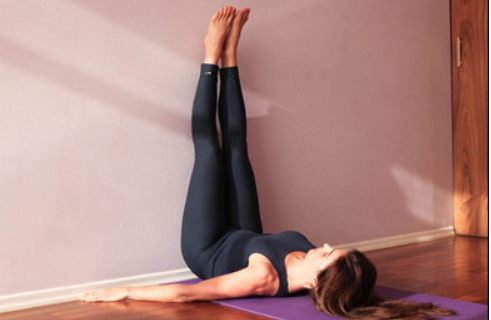
\includegraphics[width=\linewidth,keepaspectratio]{ycb1_vipartikarni}
				
				{\tiny (Ref: Yoga4Lyf)}	        
		\end{center}   
        \end{center}    
    \end{column}
  \end{columns}
\end{frame}

%%%%%%%%%%%%%%%%%%%%%%%%%%%%%%%%%%%%%%%%%%%%%%%%%%%%%%%%%%%%%%%%%%%%%%%%%%%%%%%%%%
\begin{frame}[fragile]\frametitle{Saral Matsyasana}
\begin{columns}
    \begin{column}[T]{0.5\linewidth}
      \begin{itemize}
        \item Lie on your back, legs extended.
        \item Place hands under hips for support.
        \item Lift chest and head, arching back.
        \item Keep elbows close to the floor, shoulders relaxed.
        \item Hold the position and breathe deeply.
        \item \textbf{Benefits:} Stretches chest and neck, improves posture.
        \item \textbf{Contraindications:} Avoid if you have neck or back injuries.
      \end{itemize}
    \end{column}
    \begin{column}[T]{0.5\linewidth}
        \begin{center}
        \begin{center}
		        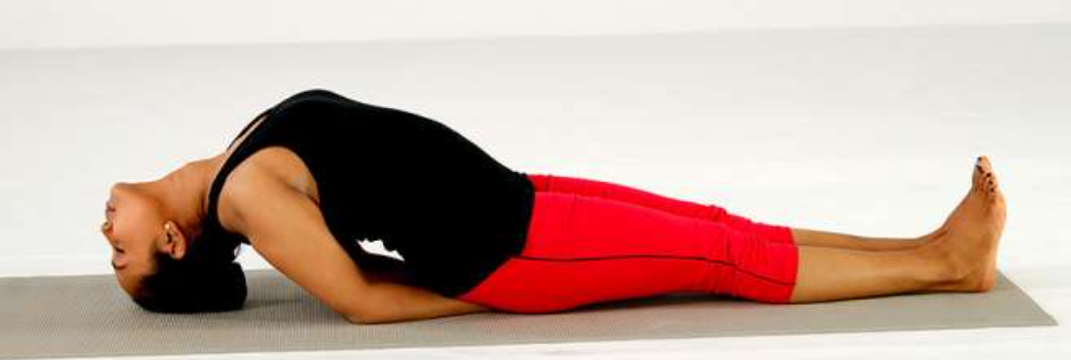
\includegraphics[width=\linewidth,keepaspectratio]{ycb1_saralmatsyasan}
				
				{\tiny (Ref: Kerala Tourism)}	        
		\end{center}   
        \end{center}    
    \end{column}
  \end{columns}
\end{frame}

